%%%%%%%%%%%%%%%%%%%%%%%%%%%%%%%%%%%%%%%%%
% Journal Article
% LaTeX Template
% Version 1.0 (25/8/12)
%
% This template has been downloaded from:
% http://www.LaTeXTemplates.com
%
% Original author:
% Frits Wenneker (http://www.howtotex.com)
%
% License:
% CC BY-NC-SA 3.0 (http://creativecommons.org/licenses/by-nc-sa/3.0/)
%
%%%%%%%%%%%%%%%%%%%%%%%%%%%%%%%%%%%%%%%%%

%----------------------------------------------------------------------------------------
%	PACKAGES AND OTHER DOCUMENT CONFIGURATIONS
%----------------------------------------------------------------------------------------

\documentclass[twoside]{article}

\usepackage{lipsum} % Package to generate dummy text throughout this template

\usepackage[sc]{mathpazo} % Use the Palatino font
\usepackage[T1]{fontenc} % Use 8-bit encoding that has 256 glyphs
\linespread{1.05} % Line spacing - Palatino needs more space between lines
\usepackage{microtype} % Slightly tweak font spacing for aesthetics

\usepackage[hmarginratio=1:1,top=32mm,columnsep=20pt]{geometry} % Document margins
\usepackage{multicol} % Used for the two-column layout of the document
\usepackage{hyperref} % For hyperlinks in the PDF

\usepackage[hang, small,labelfont=bf,up,textfont=it,up]{caption} % Custom captions under/above floats in tables or figures
\usepackage{booktabs} % Horizontal rules in tables
\usepackage{float} % Required for tables and figures in the multi-column environment - they need to be placed in specific locations with the [H] (e.g. \begin{table}[H])

\usepackage{graphicx}
\usepackage{amsmath} 
\usepackage{caption}
\usepackage{epsfig}
\usepackage{subcaption}
\usepackage{lettrine} % The lettrine is the first enlarged letter at the beginning of the text
\usepackage{paralist} % Used for the compactitem environment which makes bullet points with less space between them

\usepackage{abstract} % Allows abstract customization
\renewcommand{\abstractnamefont}{\normalfont\bfseries} % Set the "Abstract" text to bold
\renewcommand{\abstracttextfont}{\normalfont\small\itshape} % Set the abstract itself to small italic text

\usepackage{titlesec} % Allows customization of titles
\titleformat{\section}[block]{\large\scshape

\usepackage{fancyhdr} % Headers and footers
\pagestyle{fancy} % All pages have headers and footers
\fancyhead{} % Blank out the default header
\fancyfoot{} % Blank out the default footer
\fancyhead[C]{Astronomy 330 : Paper 3} % Custom header text
\fancyfoot[RO,LE]{\thepage} % Custom footer text

\usepackage{setspace}
\doublespacing
%-----New Commands


%----------------------------------------------------------------------------------------
%	TITLE SECTION
%----------------------------------------------------------------------------------------

\title{\vspace{-15mm}\fontsize{24pt}{10pt}\selectfont\textbf{Big Bang Nucleosynthesis}} % Article title

\author{
\large
\textsc{Allan Gamboa}\\ % Your name
\normalsize San Francisco State University
\vspace{-5mm}
}
\date{}

%=========================================
%=========================================
\begin{document}

\maketitle % Insert title

\thispagestyle{fancy} % All pages have headers and footers
%=========================================
%=========================================

\section{Introduction}
The very early universe  was hot and dense enough to enable fusion of elements beyond hydrogen. Bear Protons and Neutrons where combined to form everything from Deuterium to Lithium-7 in non-negligible quantities. The actual mass fractions\footnote{We note that by definintion the SUm of all mass fractions for all isotopes must add up to one.} produced, where a mass fraction for a particular isotope is defined to be,
\begin{align}
X_{i} = \frac{A_{i}n_{i}}{\rho_{b}N_{A}}
\end{align}
where $A_{i}$ is the mass number, $n_{i}$ the number density, $N_{A}$ Avogadro's number, and $\rho_{b}$ the baryon density, are very sensitive to the temperature of the system, in our case the universe.
Cosmology allows us to to predict the evolution of the temperature of the universe. Because the temperature of the universe is defined by the photons that  fill it, and the photons that fill it are those that emerge from the time of recombination or last scattering i.e the Cosmic Microwave Background (CMB). We, to a very good approximation, need to track just these photons to determine the temperature of the universe as a function of time. \par 
If we approximate the CMB to be a blackbody we can relate its energy density to its temperature via  Stefan Boltzmann's Law,
\begin{align}
&\epsilon_{rad} = \sigma T^{4}/c\quad\text{Plugging in for $\epsilon_{rad}$}\\
&\frac{\epsilon_{rad,0}}{a^{4}(t)} = \sigma T^{4}/c\quad\text{whch implies}\\
&T\propto\frac{1}{a(t)} \quad\text{Given that $a(t=today)=a(t_{0}=1)$}\\
&T=\frac{T_{0}}{a(t)} \quad\text{Where $T_{0}$ is the temperature today.}\label{eq:tofa}
\end{align}
Thus we merely need to solve for the scale factor, $a(t)$, as a function of time to know the evolution of the temperature for all time. To do this we turn to the Freedman equation,
\begin{align}
\left(\frac{\dot{a}}{a}\right)^{2} = H_{0}^{2}\left(\frac{\Omega_{M,0}}{a^{3}} + \frac{\Omega_{R,0}}{a^{4}} + \Omega_{\Lambda,0} +\frac{\Omega_{K,0}}{a^{2}} \right)
 \end{align}
 and solve for $a(t)$. In general this equation cannot be solved analytically but  under the very good approximation that during the time of interest\footnote{Alll of nucleosynteshis took place within a few thousands of seconds from the big bang. } the universe was radiation dominated, the differential equation becomes,
\begin{align}
\left(\frac{\dot{a}}{a}\right)^{2} = H_{0}^{2}\frac{\Omega_{R,0}}{a^{4}} 
 \end{align}
 Giving us,
\begin{align}
a(t) = \sqrt{2H_{0}t\sqrt{\Omega_{R,0}}}\label{eq:aoft}
\end{align}
Where $H_{0}$ is the Hubble Constant, and $\Omega_{R,0}$ is  the radiation density parameter as measured today.

For ourAnalysis we take $\Omega_{R,0} = 0.04$, $Omega_{r,0} = 8\times 10^{-5}$, $T_{0} = 2.7 [K]$ and $H_{0} = 10 [km/s\cdot Mpc]$. These values are relisted in table~\ref{t:parameters} for convenience. We reference \emph{On the Synthesis Of Elements at very HIgh Temperatures} by Wagoner et all for the reaction rates of interest and determine the Mass Fraction evolution vs time for Protons, Neutrons, Deuterium, $He^{3}$, $He^{4}$, tritium. We finally  vary $Omega_{B,0}$ to calculate  the manner in which the freeze out values change vs this parameter.


\begin{table}[h!]
  \begin{center}
    \begin{tabular}{ c | c | c | c}
    $\boldsymbol{\Omega_{B,0}}$& $\boldsymbol{\Omega_{R,0}}$ & $\boldsymbol{H_{0}}$ & $\boldsymbol{T_{0}}$ \\\hline &&&\\
    0.04 & $8\times 10^{-5}$ & $70[\frac{km}{s\cdot Mpc}]$ &2.7
    \end{tabular}
  \end{center}
  \caption{Cosmological parameters used for the calcualtions.}\label{t:parameters}
\end{table}

%===========================================
\subsection{The initial Condiitons}
For convenience we take our staring time as the time after the big bang such that the following conditions are met:
\begin{enumerate}
 \item The universe was hot enough to enable thermal equilibrium between the particles present but not so hot that the particles are relativistic (i.e. enforcing $k_{B}T<<m_{p}c^{2}$).
\item The only nucleons present at this time are bare Neutrons and Protons
\end{enumerate}
Under the thermal equilibrium requirement the number of Neutrons to Protons is given by a Maxwell Boltzmann distribution,
\begin{align}
\frac{N_{n}}{N_{p}}  = \left(\frac{m_{n}}{m_{p}}\right)^{3/2}e^{-\frac{(m_{n}-m_{p})c^{2}}{k_{B}T}}\label{eq:maxwell}
\end{align}
At a temperature of $k_{B}T\approx 0.8MeV$ the mass difference between the proton and neutron becomes non negligible and the two are no longer in thermal equilibrium. Their relative abundance is well approximated by equation~\ref{eq:maxwell} and is given by $\approx \frac{1}{5}$.\par

From this time forward neutrons are free to decay until it is cool enough that neutrons can bind with other nuclei to form more stable isotopes such as $D$, $He_{3}$ and $He_{4}$. This moment corresponds to a temperature of $\approx 0.06$[MeV] which in turn corresponds to a time from $k_{B}T \approx 0.8MeV$ of $340 [s]$, refer to  equation~\ref{eq:aoft} and equation~\ref{eq:tofa}. Given that the neutron half life is $614[s]$ the initial neutron to proton ratio we are left with is,
\begin{align}
\frac{N_{n}}{N_{p}} = \frac{1}{5}\times e^{-\frac{340[s]\times ln(2)}{614[s]}}\approx \frac{1}{7.3}
\end{align}

%===========================================
%===========================================
%===========================================

\section{Strong and electromagnetic Reactions} 
The relevant reactions where taken from \emph{On the Synthesis Of Elements at Very High Temperatures} by Wagoner et all. They are shown on figure~\ref{f:reactions} and figure~\ref{f:reactions2}, in appendix~\ref{a:reac}. All reactions except those involving 3 isotopes on the left or right hand side where taken into consideration.\par 

Referring to  figure~\ref{f:reactions} and figure~\ref{f:reactions2}, the quantities under the reactions are the rates the first quantity is the forward rate $R_{fow}$ and the backward rate $R_{back}$. Denoting the elements on the left hand side as $E_{LHS}$  and their corresponding mass fractions as $E_{LHS}$; and the elements on the right hand side as $E_{RHS}$ and their corresponding mass fractions as $E_{RHS}$, the evolution of the mass fraction for the $i^{th}$ element in the reaction is given by,
\begin{align}
&\frac{1}{A_{i}}\frac{dX_{i}}{dt} = -\sum 1/A_{j}X_{LHS,j}*R_{fow}+ \sum 1/A_{k}X_{LHS,k}*R_{back}\quad\text{if $E_{i}$ is on the Left Hand Side}\\
&\frac{1}{A_{i}}\frac{dX_{i}}{dt} = \sum 1/A_{j}X_{LHS,j}*R_{fow}-\sum 1/A_{k}X_{LHS,k}*R_{back}\quad\text{if $E_{i}$ is on the Right Hand Side}
\end{align} 
As more reactions are considered we simply add terms to the Right Hand Side of the equations above.

\begin{figure}[b!]
  \centering
	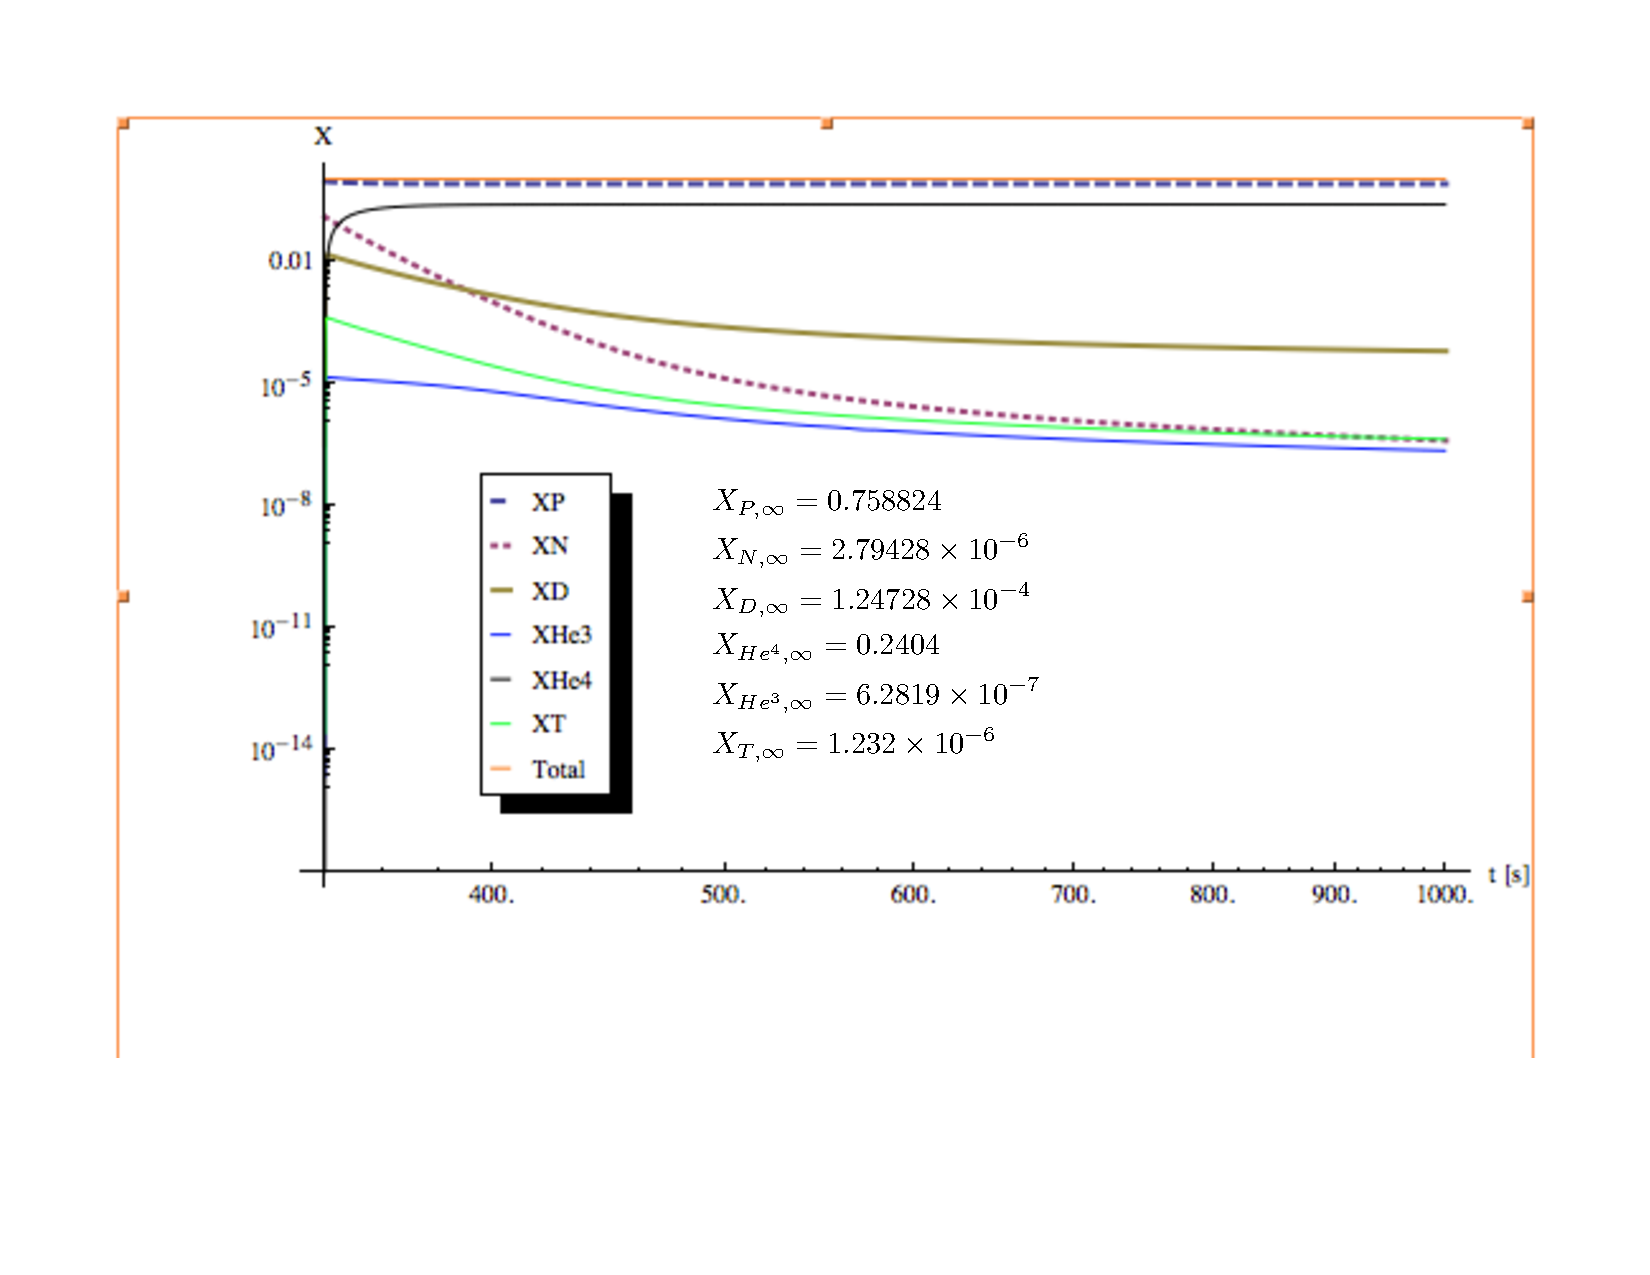
\includegraphics[width=0.8\textwidth]{fracvst.pdf}
  \caption{The evolution of the mass fraction vs ttime fopr a unvirese with the properties listed in table~\ref{t:parameters}. Listed also are the final freese out mass frations for all the isotopes involved  }\label{f:fracvst}
\end{figure}

Mathematica's NDSolve function was used to solve the six coupled first order differential equations for Protons, Neutrons, Deuterium, $He^{3}$, $He^{4}$, and Tritium with the following initial conditions at time equal to $340s$,
\begin{align}
&X_{P,0}+X_{N,0} = 1\\
&\frac{X_{P,0}}{X_{N,0}} = 7.3\\
&X_{D,0} = X_{He_{3},0} = X_{He_{4},0}=X_{T,0} = 0   
\end{align}
We also included the weak neutron decay by approximating its lifetime to be $882 [s]$.\par 

The results from this calculation is shown on figure~\ref{f:fracvst}.




%===========================================
%===========================================
%===========================================

\section{Varying $Omega_{B,0}$} 
We also varied the value of $Omega_{B,0}$ with values of $0.001$ to $0.1$ and computed the freeze out values at each. The results are plotted on figure~\ref{f:fracvsomeg1} and figure~\ref{f:fracvsomeg2}. 

\begin{figure}[h!]
  \centering
	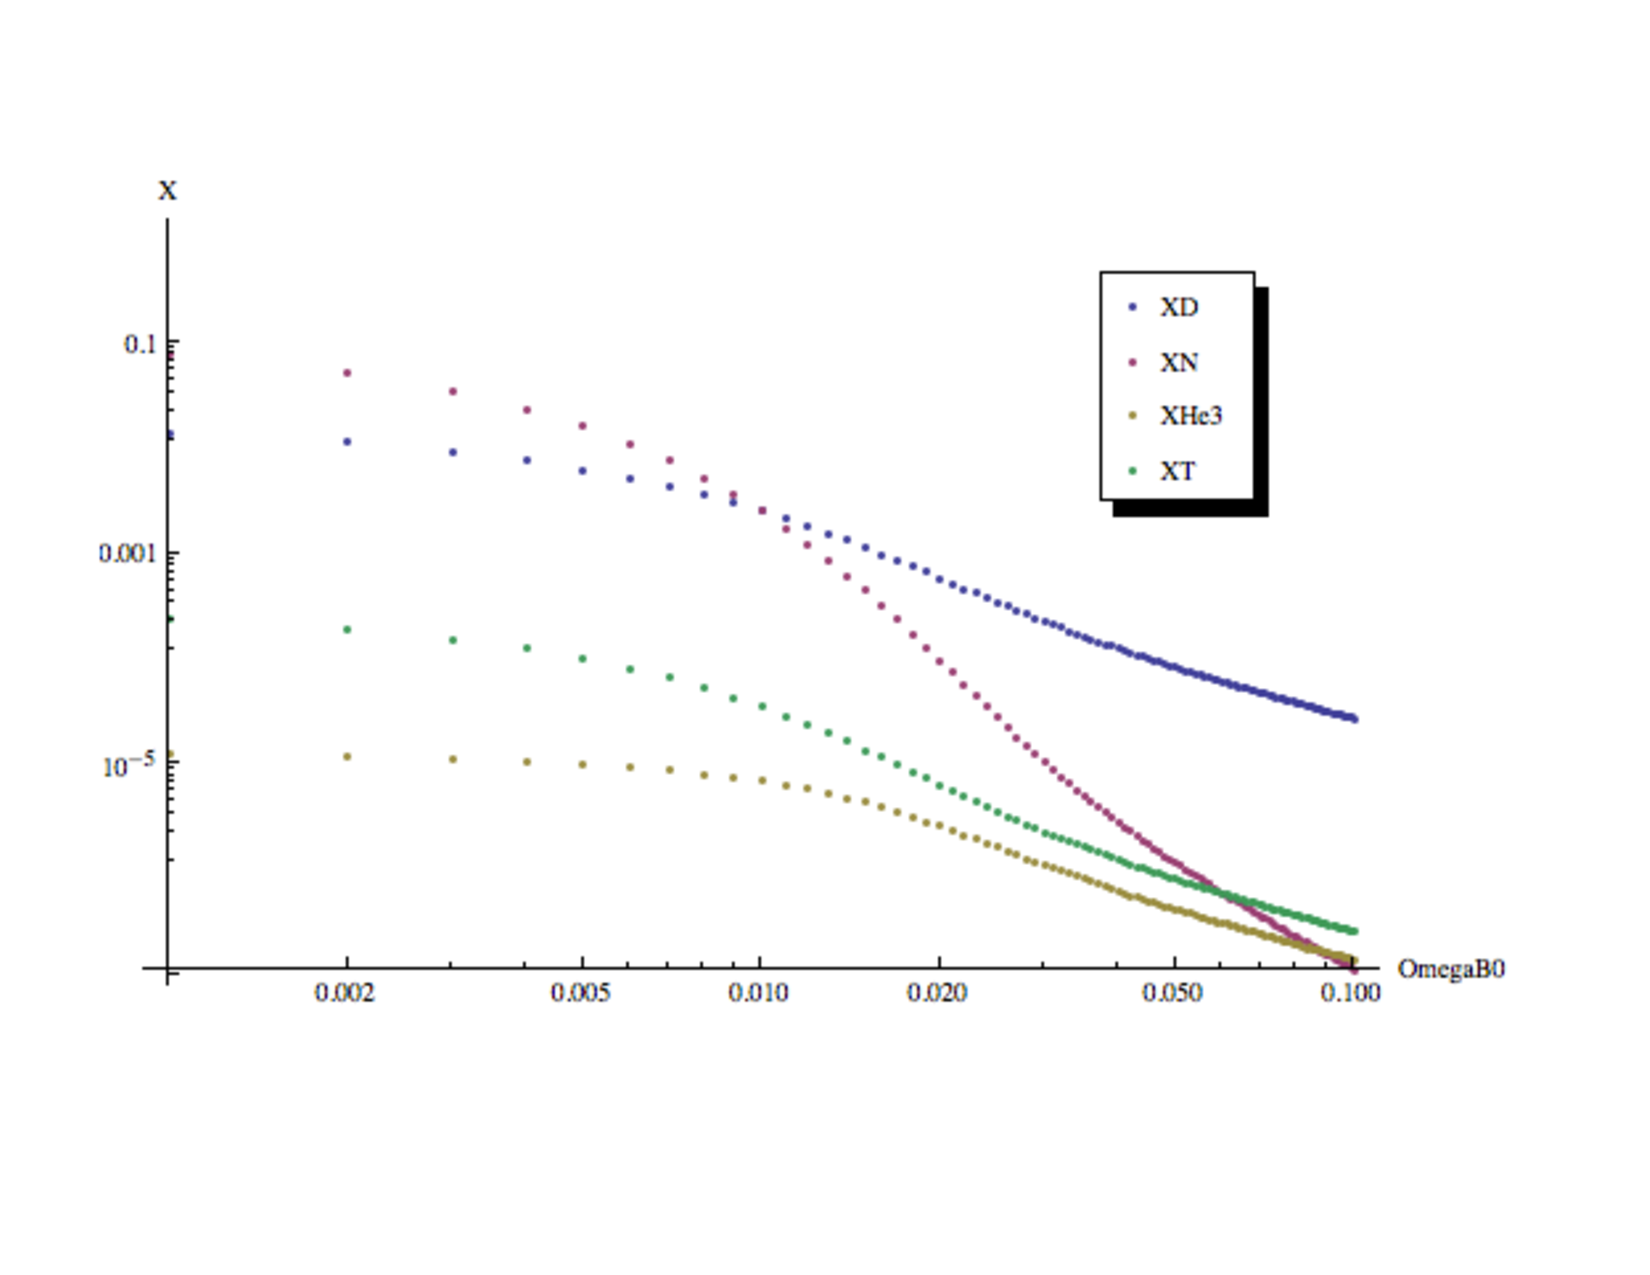
\includegraphics[width=0.9\textwidth]{fracvsomeg1.pdf}
  \caption{The evolution of the mass fraction vs time for a unvirese with the properties listed in table~\ref{t:parameters}. Listed also are the final freese out mass frations for all the isotopes involved  }\label{f:fracvsomeg1}
\end{figure}
\begin{figure}[h!]
  \centering
	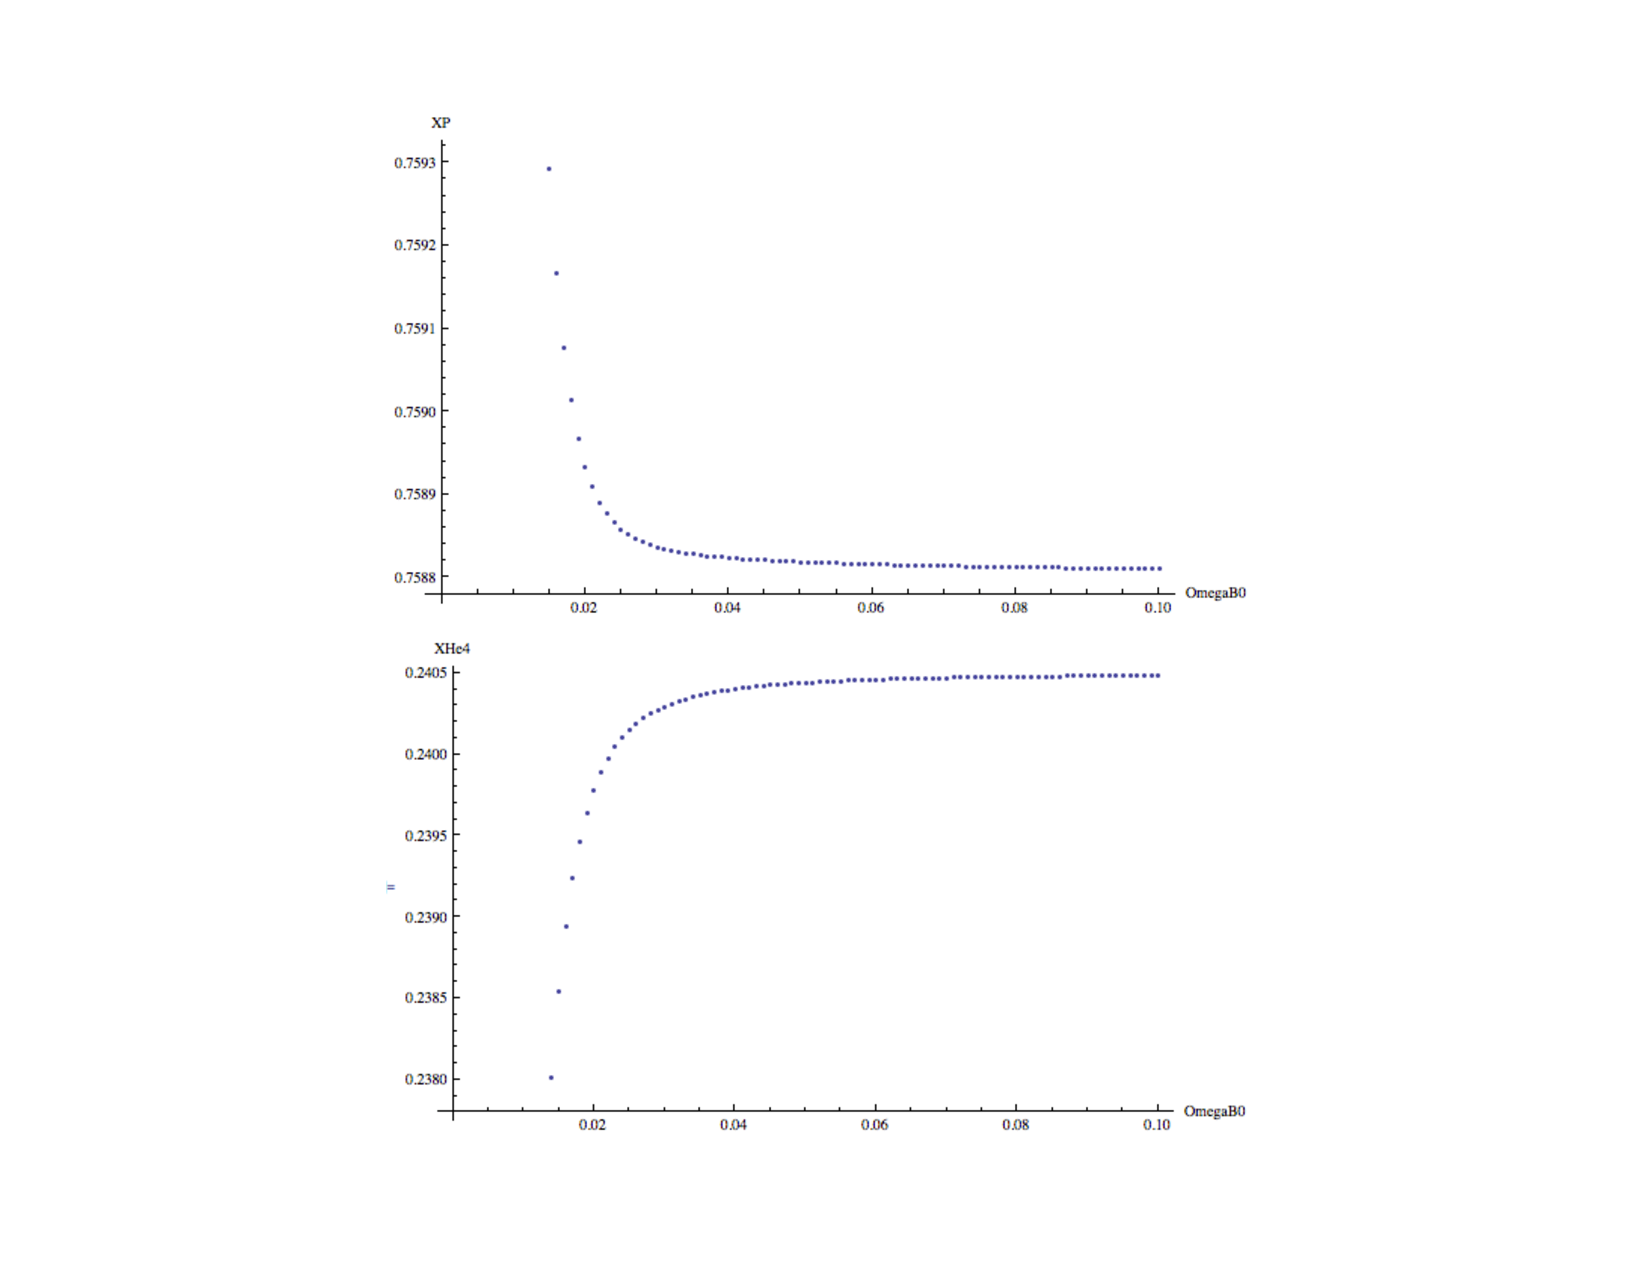
\includegraphics[width=1\textwidth]{fracvsomeg2.pdf}
  \caption{The evolution of the mass fraction vs time for a unvirese with the properties listed in table~\ref{t:parameters}.}\label{f:fracvsomeg2}
\end{figure}
Values of the final mass fractions where also sampled and portrayed in table~\ref{t:diffFracs}.

\begin{table}[h!]
  \begin{center}
    \begin{tabular}{l |l |l |l |l |l |l }
    \hline
    $\boldsymbol{\Omega_{B,0}}$ & $\boldsymbol{X_{P,\infty}}$ & $\boldsymbol{X_{N,\infty}}$ & $\boldsymbol{X_{D,\infty}}$ & $\boldsymbol{X_{He_{3},\infty}}$ & $\boldsymbol{X_{He_{4},\infty}}$ & $\boldsymbol{X_{T,\infty}}$ \\\hline
  
0.001 & 0.836334 & 0.0772533 & 0.0139512, 
 & 0.0000122267 & 0.0721095 &  0.000242501\\
0.01 & 0.761369 & 0.00249106  &  0.00253585 
 &  6.93674E-6 & 0.23306 & 0.0000352829\\
0.02 & 0.758934 & 0.0000961728 & 0.000581908 & 2.58356E-6 & 0.23978 & 6.31472E-6\\
0.03 & 0.758837 &  0.0000105211 &  0.000225343 & 1.1056E-6 & 0.240293 & 2.27072E-6\\
0.04 &  0.758824 &  2.79428E-6 & 0.000124728 
   &  6.2819E-7 &  0.2404 &  1.232E-6\\
 0.05 &  0.758819 &  1.15776E-6 &  0.0000828317
  &  4.20119E-7 &  0.24044 &  8.11364E-7\\
 0.06 & 0.758816 & 6.00474E-7 &  0.0000606641
   &  3.09628E-7 &  0.240459 &  5.90366E-7\\
 0.07 &  0.758814 &  3.56085E-7 &  0.0000472095
   &  2.41924E-7 &  0.24047 & 4.56767E-7\\
 0.08 &  0.75881 & 2.29286E-7 &  0.0000381675
   & 1.96233E-7 & 0.240476 & 3.6721E-7\\
 0.09 & 0.758811 & 1.56893E-7 &  
  0.0000317518 & 1.63716E-7 & 0.240481 & 
  3.03765E-7\\
0.1 & 0.75881 & 1.12166E-7 & 
  0.0000269685 & 1.39424E-7 &  0.240484 &  
  2.56523E-7\\
    \hline
    \end{tabular}
  \end{center}
  \caption{The mass fractions sampled at values of $\Omega_{B,0}$ between $0.001$ and $0.1$.}\label{t:diffFracs}
\end{table}




%===============================================
%===============================================
%===============================================
\pagebreak
\newpage
\section{Discusion}
It is clear that the final elemental abundances are heavily dependent  values of cosmological parameters, since the scale factor is and the temperature is in turn dependent on the scale factor. Of particular importance in big bang nucleosynthesis is $\Omega_{B,0}$. Thus by measuring elemental abundances in primordial gas that has been relatively unaltered since the end of big bang nucleosynthesis one can find via t the theory the appropriate value of $\Omega_{B,0}$. This is commonly  done by measuring deuterium abundances from quasar light as it passes through primordial gas. From the spectrum of this light one determines relative abundance by the strength of lines corresponding to deuterium with respect to other lines. These measurements suggest that $\Omega_{B,0}\approx 0.04$.
Given that this is the case and that $\sum \Omega_{i,0} = 1$ where is the rest of the mass density of the universe made of. \par
Given that CMB data along with other independent studies strongly suggest that we live in a flat universe, most of the universe must be made up of things we cannot detect and have thus dubbed "Dark." It is now believed that the universe is nearly entirely made up of dark matter and dark energy.


%========================================
%========================================
\newpage
\pagebreak
\appendix
\section{Reactions}\label{a:reac}

\begin{figure}[h!]
  \centering
      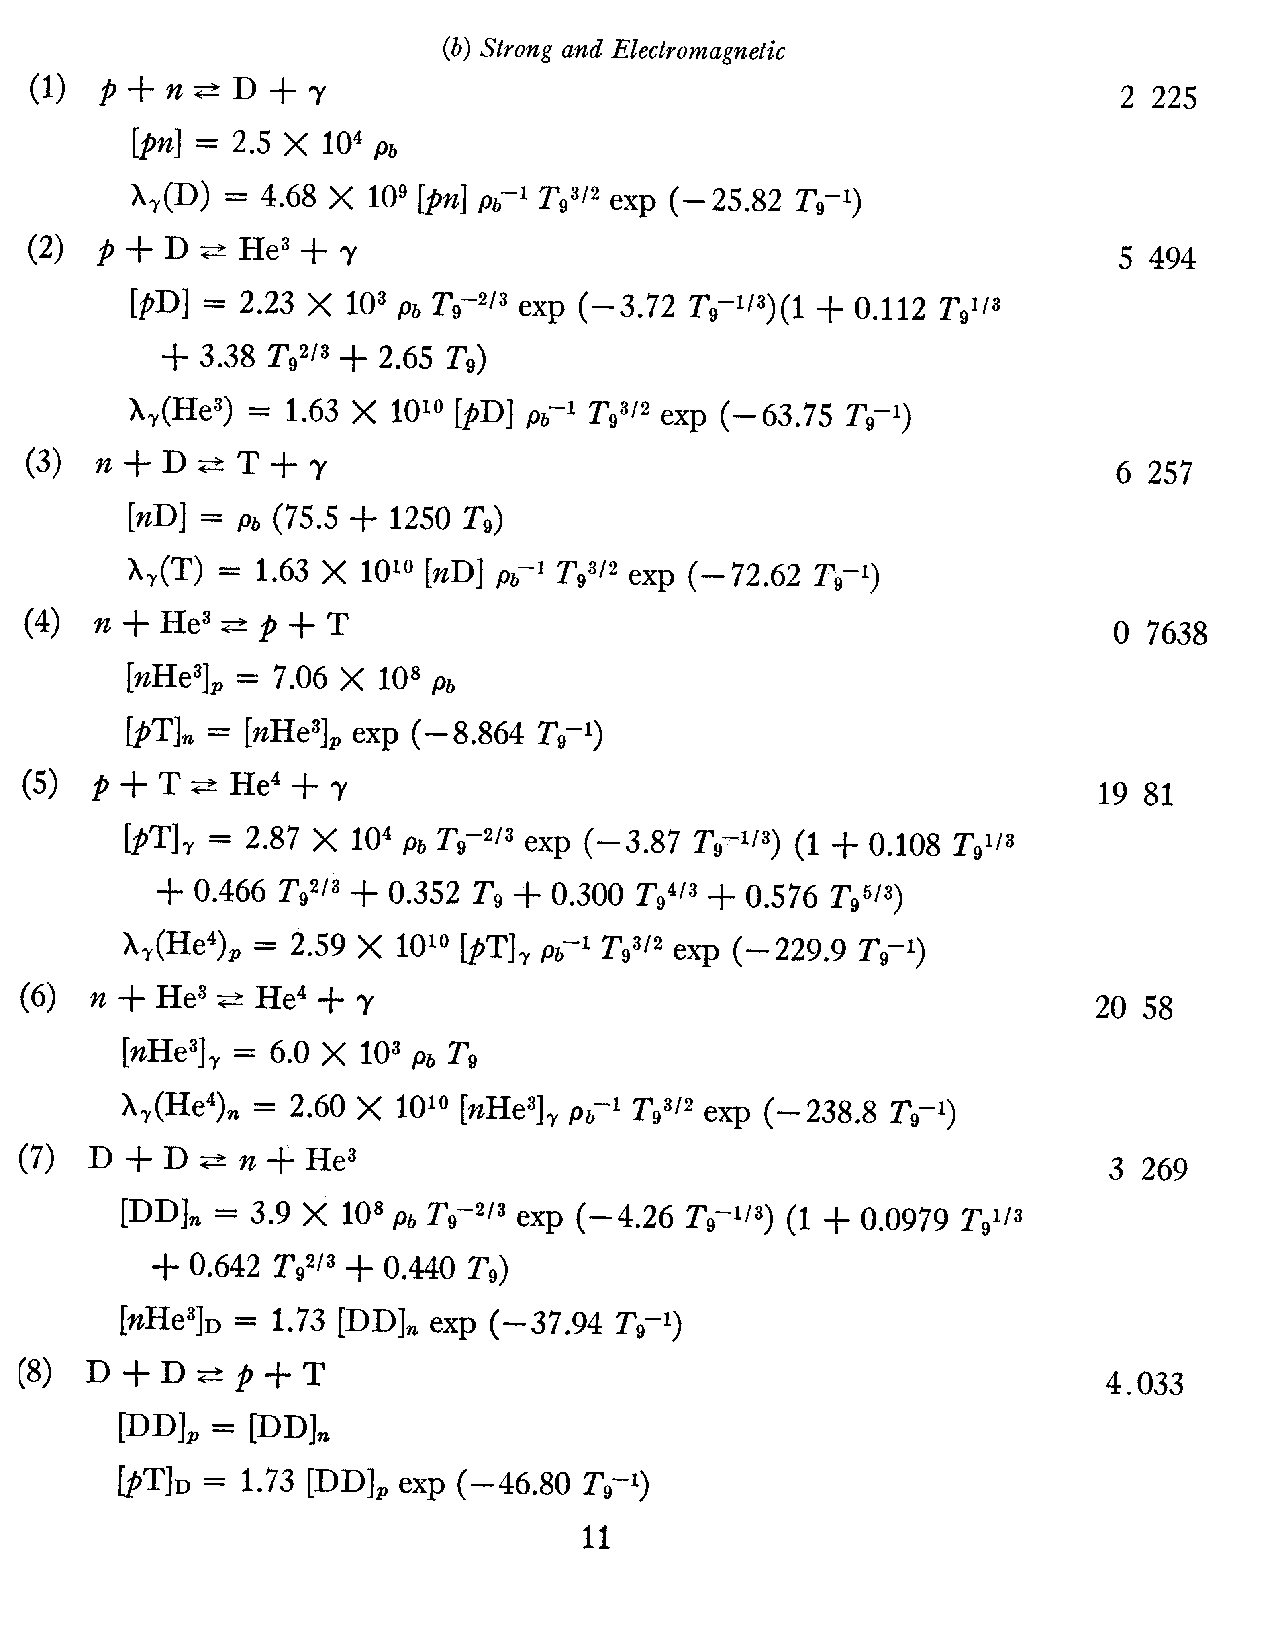
\includegraphics[width=0.9\textwidth]{eqs1.pdf}
  \caption{Strong and electromagnetic Reactions from \emph{On the Synthesis Of Elements at very HIgh Temperatures} by Wagoner et a. }\label{f:reactions}
\end{figure}
\begin{figure}[h!]
  \centering
	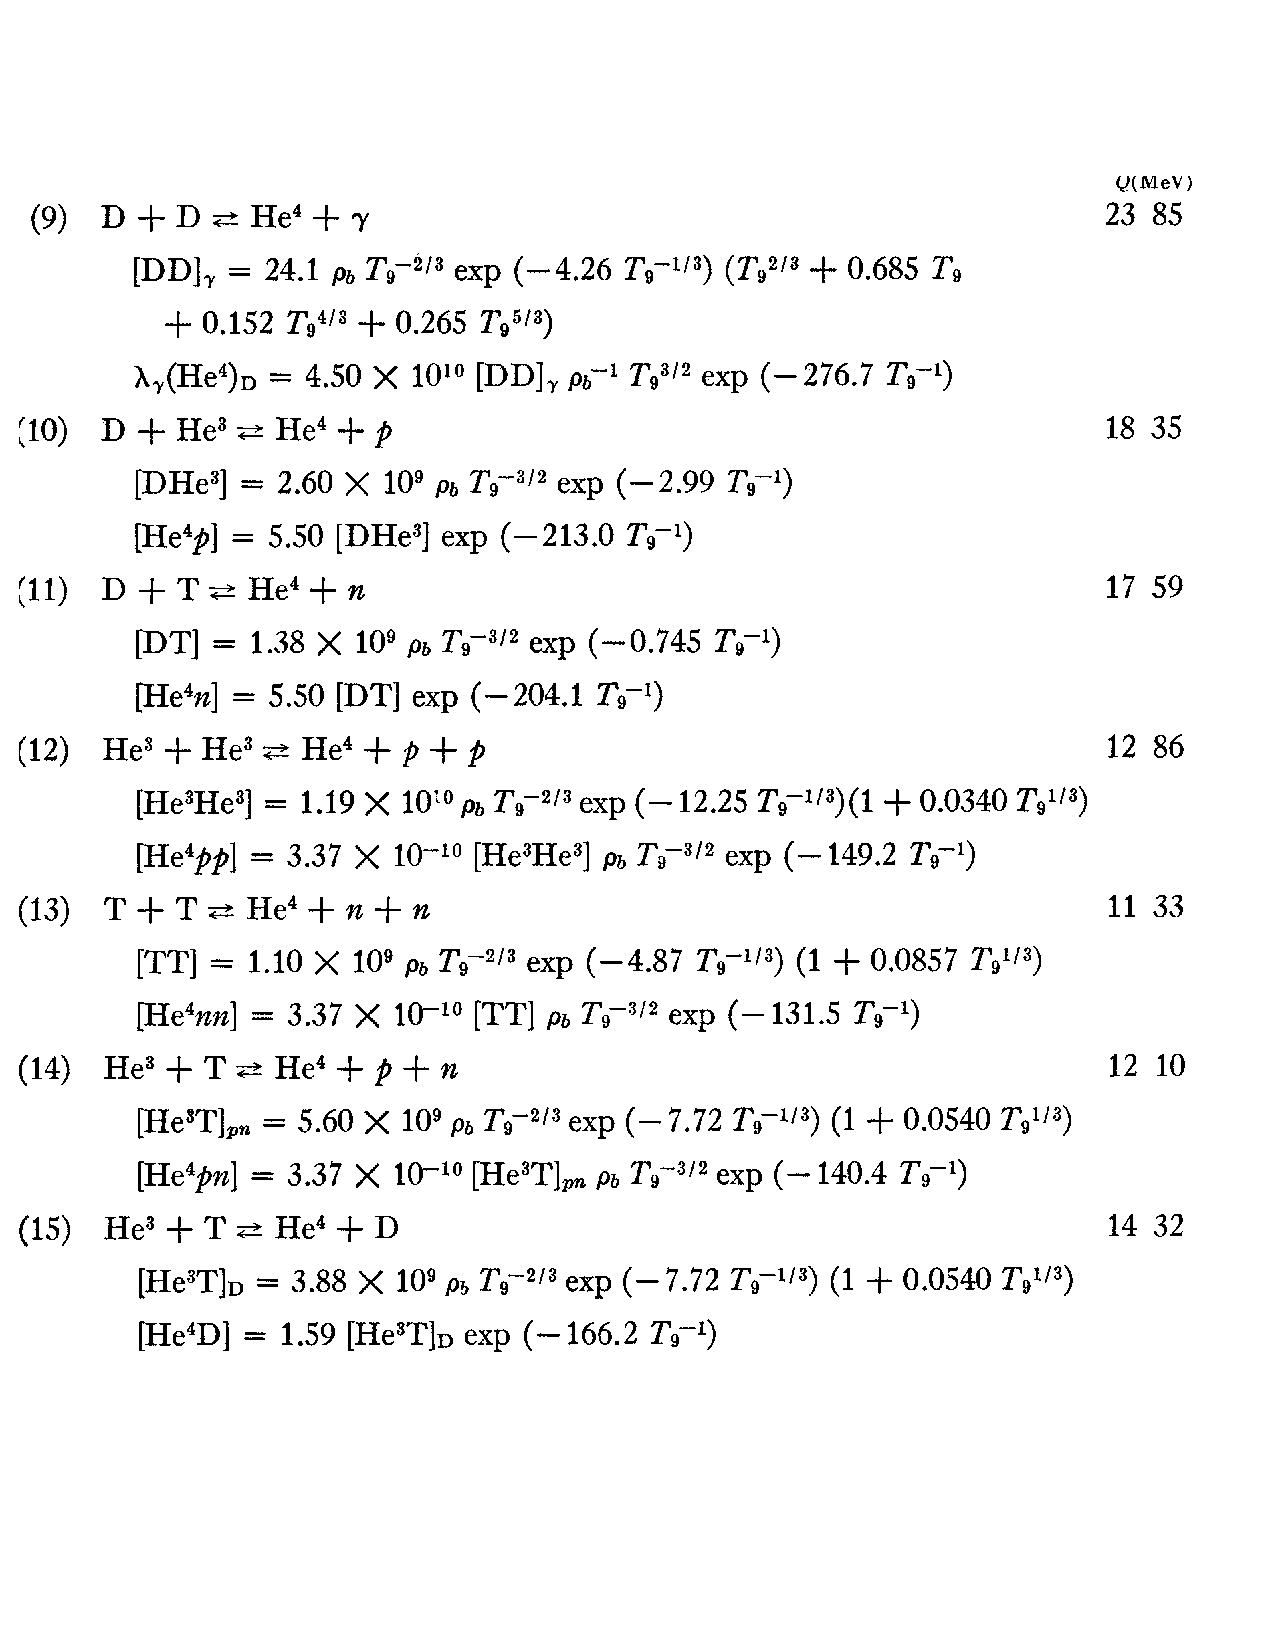
\includegraphics[width=0.9\textwidth]{eqs2.pdf}
  \caption{Strong and electromagnetic Reactions from \emph{On the Synthesis Of Elements at very HIgh Temperatures} by Wagoner et a. }\label{f:reactions2}
\end{figure}
\newpage

Here $T_{g}$ is the temperature of the universe, and $rho_{b}$ is the baryon density which is related to the baryon density parameter in the following manner,
\begin{align}
\rho_{b}(t) = \frac{3H_{0}}{8\pi G}\Omega_{b,0}
\end{align}
The rates depend on these parameters since the the greater the baryon density the  the more likely particles are to interact and the greater the temperature the more likely they are to overcome the coulomb barrier. This is an overtly simplified explanation, the exact form of the rates takes into account statistical and quantum mechanical nature of interactions in an effort to compute interaction cross-ssections. A rate is given by,
\begin{align}
R_{i} = \rho_{b}N_{A}\langle\sigma v\rangle_{i}
\end{align}
Where $\sigma$ is the interaction cross-section and $v$ is the velocity of the particle.





%=======================================

\end{document}




%---------------------------------------------------



\begin{figure}[h!]
  \centering
      \includegraphics[width=0.5\textwidth]{gull}
  \caption{A picture of the same gull
           looking the other way!}
\end{figure}
 #==================================================


\begin{table}[h!]
  \begin{center}
    \begin{tabular}{| l c r |}
    \hline
    1 & 2 & 3 \\
    4 & 5 & 6 \\
    7 & 8 & 9 \\
    \hline
    \end{tabular}
  \end{center}
  \caption{A simple table}
\end{table}
#========================================================

\usepackage{graphicx}
\usepackage{caption}
\usepackage{subcaption}
 
\begin{figure}
        
        \begin{subfigure}[b]{0.3\textwidth}
                \centering
                \includegraphics[scale=.5]{MagVsTg.pdf}
                \caption{A gull}
                \label{fig:gull}
        \end{subfigure}%
        \hspace{3cm} %add desired spacing between images, e. g. ~, \quad, \qquad etc. 
          %(or a blank line to force the subfigure onto a new line)
        \begin{subfigure}[b]{0.3\textwidth}
                \centering
                \includegraphics[scale=.5]{MagVsTi.pdf}
                \caption{A tiger}
                \label{fig:tiger}
        \end{subfigure}
        ~ %add desired spacing between images, e. g. ~, \quad, \qquad etc. 
          %(or a blank line to force the subfigure onto a new line)
	\\
        \begin{subfigure}[b]{0.3\textwidth}
                \centering
                \includegraphics[scale=.5]{MagVsTr.pdf}
                \caption{A mouse}
                \label{fig:mouse}
        \end{subfigure}
	\hspace{3cm} %add desired spacing between images, e. g. ~, \quad, \qquad etc. 
          %(or a blank line to force the subfigure onto a new line)
        \begin{subfigure}[b]{0.3\textwidth}
                \centering
                \includegraphics[scale=.5]{MagVsTu.pdf}
                \caption{A mouse}
                \label{fig:mouse}
        \end{subfigure}
	\\
        \begin{subfigure}[b]{0.3\textwidth}
                \centering
                \includegraphics[scale=.5]{MagVsTz.pdf}
                \caption{A mouse}
                \label{fig:mouse}
        \end{subfigure}

        \caption{Absolute Magnitude Vs Time}\label{fig:animals}

\end{figure}
